\documentclass[a4paper]{article}

\usepackage[utf8]{inputenc}
\usepackage[T1]{fontenc}     
\usepackage[francais]{babel}  
\usepackage[top=5cm, bottom=5cm, left=3cm, right=3cm]{geometry}
\usepackage{graphicx} 
\usepackage{graphics} 
\usepackage{float}

\title{Les fractales}
\author{Stephanie \bsc{Noel} et Sid \bsc{Berraf}}
\date{\today}

\begin{document}
\maketitle
\newpage
\tableofcontents
\newpage

\section{Introduction}
Les premiers exemples de fractals remontent à la Grèce Antique : la ``baderne d’Apollonius `` est le plus ancien exemple de fractal, datant d’Apollonius de Perge, 3ème siècle avant J.C. : c'est aussi lui qui donna à l'ellipse, à la parabole et à l'hyperbole les noms que nous connaissons aujourd’hui.\\\\\

\begin{figure}[H]
\begin{center}
\includegraphics[width=6cm]{./../doc/Sans-titre-1.png}
\end{center}
\end{figure}

Les secteurs artistiques, et notamment la peinture, ont aussi leurs parts de fractals, et ce depuis bien longtemps. Ainsi dans les peintures de Katsushika Hokusai, un peintre japonais du surnom de “Vieux Fou de la peinture”, on peut observer des motifs fractals. Comme par exemple dans La Grande Vague de Kanagawa,, On peut en effet observer que la vague principale se termine par des vaguelettes identiques.\\\\

\begin{figure}[H]
\begin{center}
\includegraphics[width=6cm]{./../doc/Sans-titre-3.jpg}
\end{center}
\end{figure}

Plus récemment, les poussières de Cantor en 1890, et  le flocon de Von Koch en 1904, firent leurs apparitions. Ces objets fractals qui apparurent bien avant l’invention de ce terme ont étés créés par des mathématiciens, mais eux même ne savent pas trop ce qu’ils représentent, comment ils pourraient être définis … d’où leur nom de “courbes monstrueuses”.\\\\

\begin{figure}[H]
\begin{center}
\includegraphics[width=3.5cm]{./../doc/Sans-titre-4.jpg}
\end{center}
\end{figure}

Un autre mathématicien précurseur de la conception de fractals se demanda pendant la Première Guerre Mondiale qu’est ce que cela donnerait si l’on appliquait une fonction quelconque et que l’on l’applique en boucle, autrement dit que l’on prenne une fonction (par ex f(x)= ax+b), que l’on l’applique à une valeur, ce qui nous donne une deuxième valeur, puis que l’on applique de nouveau cette fonction à cette deuxième valeur : on obtient alors une troisième valeur et on applique cela à l’infini. Mais bien évidement, pour l’époque il était impossible de faire cela par manque de moyen ; en effet, il est nécessaire pour cela d’avoir accès à un puissant ordinateur. Ce que fit Benoît Mandelbrot des années plus tard grâce à son poste chez IBM. Mais Benoît Mandelbrot ira plus loin encore en créant son propre ensemble qui englobe tout les ensembles de Julia. Cette ensemble est devenu l’emblème des fractals.\\

Il désigne d'un nouveau nom: les «fractales». Ce mot, qui se rapproche de «fractionné», «fragmenté», «fracturé», est à relier à une notion élémentaire et importante: l'homothétie interne, qui fournit un outil simple pour construire ces objets, étudier leur degré de complexité et déboucher sur la notion de dimension non entière, ou fractale. \\\\

\newpage
\section{Les fractales en général}
\subsection{Définition}
Une figure fractale, est une figure géométrique de structure complexe dont la création ou la forme met en jeu des règles utilisant le fractionnement, c'est à dire en suivant des règles déterministes ou stochastiques.\\\\
Plus simplement c'est un objet géométrique obtenu par exploration du comportement d'une fonction en chaque point. \\
Elle désigne des objets dont la structure est invariante par changement d'échelle. \\

\subsection{Caractéristiques}
\subsubsection{Autosimilarité}
En géométrie, "similaire" signifie quelque chose de vraiment spécifique. Des figures géométriques sont semblables s'ils ont la même forme sans forcement avoir la même taille.\\

Par exemple :
\begin{center}
Ces deux carrés sont similaires.
\begin{figure}[H]\begin{center}
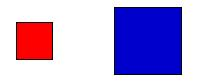
\includegraphics[width=4cm]{squares.jpg}
\end{center}
\end{figure}

Ces deux rectangles ne sont pas similaires.
\begin{figure}[H]\begin{center}
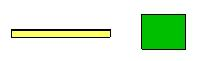
\includegraphics[width=4cm]{rec.jpg}
\end{center}
\end{figure}

Mais c'est deux rectangles le sont.
\begin{figure}[H]\begin{center}
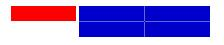
\includegraphics[width=4cm]{srec.jpg}
\end{center}
\end{figure}
\end{center}

On parle de figures autosimilaires lorsque l'ensemble de plusieurs figures identiques forment cette même figure en plus grand.
Un objet autosimilaire est exactement ou partiellement similaire à une part de lui même.

Quelques exemples de figures autosimilaires :

\begin{figure}[H]
\begin{center}
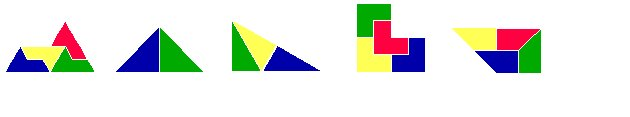
\includegraphics[width=8cm]{figures.jpg}
\end{center}
\end{figure}

\subsubsection{Dimension non entière}

On sait que qu'un point est une figure de dimension 0 ; qu'une ligne droite est un objet de dimension 1 ; qu'une surface plane est un objet de dimension 2 ; qu'un volume est de dimension 3...

Soit si on prend un segment, un carré et un cube et que l'on double leurs tailles, on obtient :

\begin{center}
Pour le segment deux copies du segment original.
\begin{figure}[H]
\begin{center}
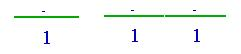
\includegraphics[width=4cm]{diseg.jpg}
\end{center}
\end{figure}
Pour le carré quatre copies.
\begin{figure}[H]
\begin{center}
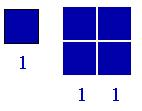
\includegraphics[width=2cm]{disq.jpg}
\end{center}
\end{figure}
Et pour le cube huit copies.
\begin{figure}[H]
\begin{center}
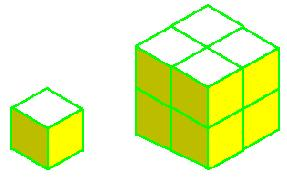
\includegraphics[width=2cm]{dicu.jpg}
\end{center}
\end{figure}
\end{center}

Il apparait donc que lorsque l'on double la taille des figures on obtient un nombre de copies égal à \begin{math} 2^{d} \end{math} avec d la dimension de la figure. \\
\begin{center}
\begin{tabular}{|c|c|c|} 
\hline
Figure & Dimension & Nb de copies \\
\hline
Segment & 1 & \begin{math} 2 = 2^1 \end{math} \\
Carré & 2 & \begin{math} 4 = 2^2 \end{math}\\
Cube & 3 &  \begin{math} 8 = 2^3 \end{math}\\
Figure & d & \begin{math} 2^{d} \end{math}\\
\hline
\end{tabular}
\end{center}
Maintenant, prenons un objet fractal comme le triangle de Sierpinski et doublons sa taille :

\begin{figure}[H]
\begin{center}
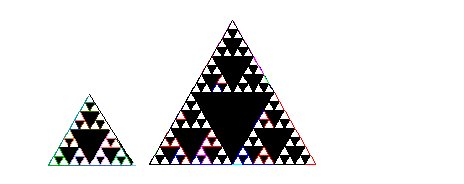
\includegraphics[width=7cm]{tri.jpg}
\end{center}
\end{figure}

On obtient trois copies (celui du milieu étant vide on ne le compte pas), donc on a \begin{math} 3 = 2^{d} \end{math} soit d entre 1,5 et 1,6.\\

Les fractales ont donc des dimensions non entières.

\subsubsection{Formation par itération}
Les fractales sont souvent formées par ce que l'on appelle un procédé d'itération.\\
Pour faire une fractale, on peut prendre une simple figure géométrique comme un triangle ou un segment, et lui appliquer une transformation qui donne une figure plus ``compliqué'' d'une certaine manière.\\
Puis, de la même manière, en répétant ce procédé à la nouvelle figure, on obtient une nouvelle figure plus ``compliqué'' et ainsi de suite... \\
On peut voir apparaître une fractale selon la transformation choisie.\\\\
Le meilleur exemple est le « flocon de neige de von Koch ».
Il s'obtient en appliquant à chaque côté d'un triangle équilatéral une transformation simple : on remplace le 1/3 central de chaque côté par 2 segments ayant la même longueur que celle qui a été prélevée et on recommence la même opération sur chaque côté de la figure obtenue. 

\begin{figure}[H]
\begin{center}
\includegraphics[width=11cm]{./../doc/flocon.png}
\end{center}
\end{figure}

À la première itération, on obtient une image proche d'une étoile de David, puis au fur et à mesure des itérations successives le résultat mime plus ou moins un flocon de neige.
\newpage

\section{Conclusion}



\end{document}
